{
\begin{table}[h!]
    \centering
    \begin{tabular}{|p{3cm}|p{15cm}|} 
        \hline
        \rowcolor{TableBgRowColor}        
        \cellcolor{HighVulnColor} \textbf{CWE} & 
        \textbf{\href{https://cwe.mitre.org/data/definitions/522.html}{CWE-522} } \\
        \hline
        \rowcolor{TableBgRowIntemediaColor}
        \cellcolor{HighVulnColor} \textbf{CVSS 3.1 Score} & 
        \textbf{9.5} \\
        \hline
        \rowcolor{TableBgRowColor}
        \cellcolor{HighVulnColor} \textbf{Impact} & 
        \textbf{9.5 (AV:N/AC:L/PR:N/UI:N/S:U/C:H/I:H/A:H)} \\
        \hline
        \rowcolor{TableBgRowIntemediaColor}        
        \cellcolor{HighVulnColor} \textbf{Description (Incl. Root
Cause)} & 
        \textbf{By responding to LLMNR/NBT-NS network traffic} \\
        \hline        
        \rowcolor{TableBgRowColor}        
        \cellcolor{HighVulnColor} \textbf{Security Impact} & 
        \textbf{Adversaries can spoof an authoritative } \\
        \hline
        \rowcolor{TableBgRowIntemediaColor}        
        \cellcolor{HighVulnColor} \textbf{Affected Domain} & 
        \textbf{INLANEFREIGHT.LOCAL} \\
        \hline
        \rowcolor{TableBgRowColor}        
        \cellcolor{HighVulnColor} \textbf{Remediation} & 
        \textbf{Disable LLMNR and NetBIOS in local computer security settings or by group policy if
they are not needed within an environment
 Use host-based security software to block LLMNR/NetBIOS traffic. Enabling SMB
Signing can stop NTLMv2 relay attacks.
 Network intrusion detection and prevention systems that can identify traffic patterns
indicative of MiTM activity can be used to mitigate activity at the network level.
 Network segmentation can be used to isolate infrastructure components that do not
require broad network access. This may mitigate, or at least alleviate, the scope of
MiTM activity} \\
        \hline
        \rowcolor{TableBgRowIntemediaColor}        
        \cellcolor{HighVulnColor} \textbf{External References} & 
        \textbf{\url{https://attack.mitre.org/techniques/T1557/001/}} \\
        \hline
    \end{tabular}
\end{table}



\begin{table}[h!]
    \centering
    \begin{tabular}{|p{3cm}|p{15cm}|} 
        \hline
        \rowcolor{TableBgRowColor}        
        \cellcolor{MediumVulnColor} \textbf{CWE} & 
        \textbf{\href{https://cwe.mitre.org/data/definitions/522.html}{CWE-522} } \\
        \hline
        \rowcolor{TableBgRowIntemediaColor}
        \cellcolor{MediumVulnColor} \textbf{CVSS 3.1 Score} & 
        \textbf{9.5} \\
        \hline
        \rowcolor{TableBgRowColor}
        \cellcolor{MediumVulnColor} \textbf{Impact} & 
        \textbf{9.5 (AV:N/AC:L/PR:N/UI:N/S:U/C:H/I:H/A:H)} \\
        \hline
        \rowcolor{TableBgRowIntemediaColor}        
        \cellcolor{MediumVulnColor} \textbf{Description (Incl. Root
Cause)} & 
        \textbf{By responding to LLMNR/NBT-NS network traffic} \\
        \hline        
        \rowcolor{TableBgRowColor}        
        \cellcolor{MediumVulnColor} \textbf{Security Impact} & 
        \textbf{Adversaries can spoof an authoritative } \\
        \hline
        \rowcolor{TableBgRowIntemediaColor}        
        \cellcolor{MediumVulnColor} \textbf{Affected Domain} & 
        \textbf{INLANEFREIGHT.LOCAL} \\
        \hline
        \rowcolor{TableBgRowColor}        
        \cellcolor{MediumVulnColor} \textbf{Remediation} & 
        \textbf{Disable LLMNR and NetBIOS in local computer security settings or by group policy if
they are not needed within an environment
 Use host-based security software to block LLMNR/NetBIOS traffic. Enabling SMB
Signing can stop NTLMv2 relay attacks.
 Network intrusion detection and prevention systems that can identify traffic patterns
indicative of MiTM activity can be used to mitigate activity at the network level.
 Network segmentation can be used to isolate infrastructure components that do not
require broad network access. This may mitigate, or at least alleviate, the scope of
MiTM activity} \\
        \hline
        \rowcolor{TableBgRowIntemediaColor}        
        \cellcolor{MediumVulnColor} \textbf{External References} & 
        \textbf{\url{https://attack.mitre.org/techniques/T1557/001/}} \\
        \hline
    \end{tabular}
\end{table}


Finding Evidence: \\
\textbf{Running the Responder tool to attempt to obtain user account password hashes.} \\

\begin{figure}[H]
    \centering
    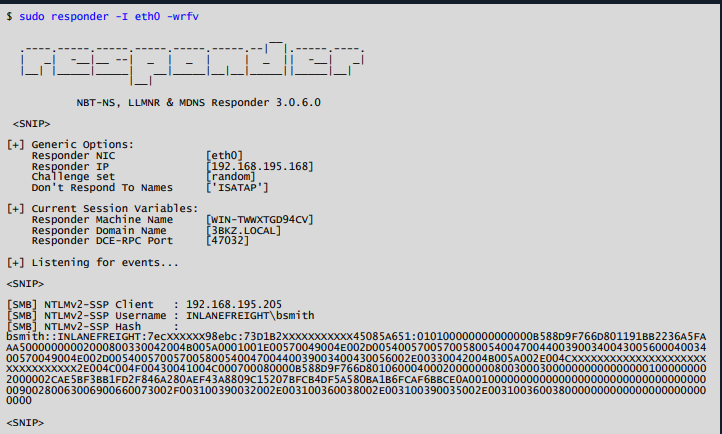
\includegraphics[width=1\linewidth]{initial//evidenceimages/responder.png}
    \caption{Enter Caption}
    \label{fig:enter-label}
\end{figure}

\textbf{Successfully cracking a password hash with Hashcat to reveal the clear text password value.}





%LOW
\begin{table}[h!]
    \centering
    \begin{tabular}{|p{3cm}|p{15cm}|} 
        \hline
        \rowcolor{TableBgRowColor}        
        \cellcolor{LowVulnColor} \textbf{CWE} & 
        \textbf{\href{https://cwe.mitre.org/data/definitions/522.html}{CWE-522} } \\
        \hline
        \rowcolor{TableBgRowIntemediaColor}
        \cellcolor{LowVulnColor} \textbf{CVSS 3.1 Score} & 
        \textbf{9.5} \\
        \hline
        \rowcolor{TableBgRowColor}
        \cellcolor{LowVulnColor} \textbf{Impact} & 
        \textbf{(AV:N/AC:L/PR:N/UI:N/S:U/C:H/I:H/A:H)} \\
        \hline
        \rowcolor{TableBgRowIntemediaColor}        
        \cellcolor{LowVulnColor} \textbf{Description (Incl. Root
Cause)} & 
        \textbf{By responding to LLMNR/NBT-NS network traffic} \\
        \hline        
        \rowcolor{TableBgRowColor}        
        \cellcolor{LowVulnColor} \textbf{Security Impact} & 
        \textbf{Adversaries can spoof an authoritative } \\
        \hline
        \rowcolor{TableBgRowIntemediaColor}        
        \cellcolor{LowVulnColor} \textbf{Affected Domain} & 
        \textbf{INLANEFREIGHT.LOCAL} \\
        \hline
        \rowcolor{TableBgRowColor}        
        \cellcolor{LowVulnColor} \textbf{Remediation} & 
        \textbf{Disable LLMNR and NetBIOS in local computer security settings or by group policy if
they are not needed within an environment
 Use host-based security software to block LLMNR/NetBIOS traffic. Enabling SMB
Signing can stop NTLMv2 relay attacks.
 Network intrusion detection and prevention systems that can identify traffic patterns
indicative of MiTM activity can be used to mitigate activity at the network level.
 Network segmentation can be used to isolate infrastructure components that do not
require broad network access. This may mitigate, or at least alleviate, the scope of
MiTM activity} \\
        \hline
        \rowcolor{TableBgRowIntemediaColor}        
        \cellcolor{LowVulnColor} \textbf{External References} & 
        \textbf{\url{https://attack.mitre.org/techniques/T1557/001/}} \\
        \hline
    \end{tabular}
\end{table}

}

